\documentclass[12pt,titlepage]{article}
\usepackage[margin=1.25in]{geometry}
\usepackage{graphicx,amsmath,blindtext}

%% Variables definition
\newcommand{\vSubject}{Project Management}
\newcommand{\vSubtitle}{Quiz 1}
\newcommand{\vName}{Dicha Zelianivan Arkana}
\newcommand{\vNIM}{2241720002}
\newcommand{\vClass}{2i}
\newcommand{\vDepartment}{Information Technology}
\newcommand{\vStudyProgram}{D4 Informatics Engineering}

%% [START] Tikz related stuff
\usepackage{tikz}
\usetikzlibrary{svg.path,calc,shapes.geometric,shapes.misc}
\tikzstyle{terminator} = [rectangle, draw, text centered, rounded corners = 1em, minimum height=2em]
\tikzstyle{preparation} = [chamfered rectangle, chamfered rectangle sep=0.75em, draw, text centered, minimum height = 2em]
\tikzstyle{process} = [rectangle, draw, text centered, minimum height=2em]
\tikzstyle{decision} = [diamond, aspect=2, draw, text centered, minimum height=2em]
\tikzstyle{data}=[trapezium, draw, text centered, trapezium left angle=60, trapezium right angle=120, minimum height=2em]
\tikzstyle{connector} = [line width=0.25mm,->]
%% [END] Tikz related stuff

%% [START] Fancy header related stuff
\usepackage{fancyhdr}
\pagestyle{fancy}
\setlength{\headheight}{15pt} % compensate fancyhdr style
\fancyhead{}
\fancyfoot{}
\fancyfoot[L]{\thepage}
\fancyfoot[R]{\textit{\vSubject - \vSubtitle}}
\renewcommand{\footrulewidth}{0.4pt}% default is 0pt, overline for footer
%% [END] Fancy header related stuff

%% [START] Custom tabular command related stuff
\usepackage{tabularx}
\newcommand{\details}[2]{
    #1 & #2  \\
}
%% [END] Custom tabular command related stuff

%% [START] Figure related stuff
\newcommand{\image}[3][1]{
    \begin{figure}[h]
        \centering
        \includegraphics[#1]{#2}
        \caption{#3}
        \label{#3}
    \end{figure}
}
%% [END] Figure related stuff

\begin{document}
\begin{titlepage}
    \centering
    \vfill
    {\bfseries\LARGE
        \vSubject\\
        \vskip0.25cm
        \vSubtitle
    }
    \vfill
    
\includegraphics[width=6cm]{images/polinema-logo.png}
    \vfill
    {
        \textbf{Name}\\
        \vName\\
        \vskip0.5cm
        \textbf{NIM}\\
        \vNIM\\
        \vskip0.5cm
        \textbf{Class}\\
        \vClass\\
        \vskip0.5cm
        \textbf{Department}\\
        \vDepartment\\
        \vskip0.5cm
        \textbf{Study Program}\\
        \vStudyProgram
    }
\end{titlepage}

\section{Quiz 1}
\begin{enumerate}
    \item {
        Jelaskan dengan detail tentang mekanisme dalam pelaksanaan proyek.
        Sertakan bagan untuk memvisualisasikan mekanisme pelaksanaan tersebut.
        \begin{itemize}
            \item The project starts from an idea from a Project Owner
            \item The Project Owner will make a Project Proposal to find sponsors for the project
            \item If the project proposal is approved, the Project Owner will make a Project Charter
            \item The Project Owner will find a Project Manager to manage the project
            \item The Developer team will be formed by the Project Manager
            \item The Project Manager will make a Project Implementation Plan
            \item Each members of the Developer team will be assigned to their respective tasks
            \item The project manager will monitor the progress of the project and report it to the Project Owner
            \item When the project is in the execution phase, it will be monitored by the Quality Assurance team
            \item If the project is finished, the Project Manager will make a report
        \end{itemize}
        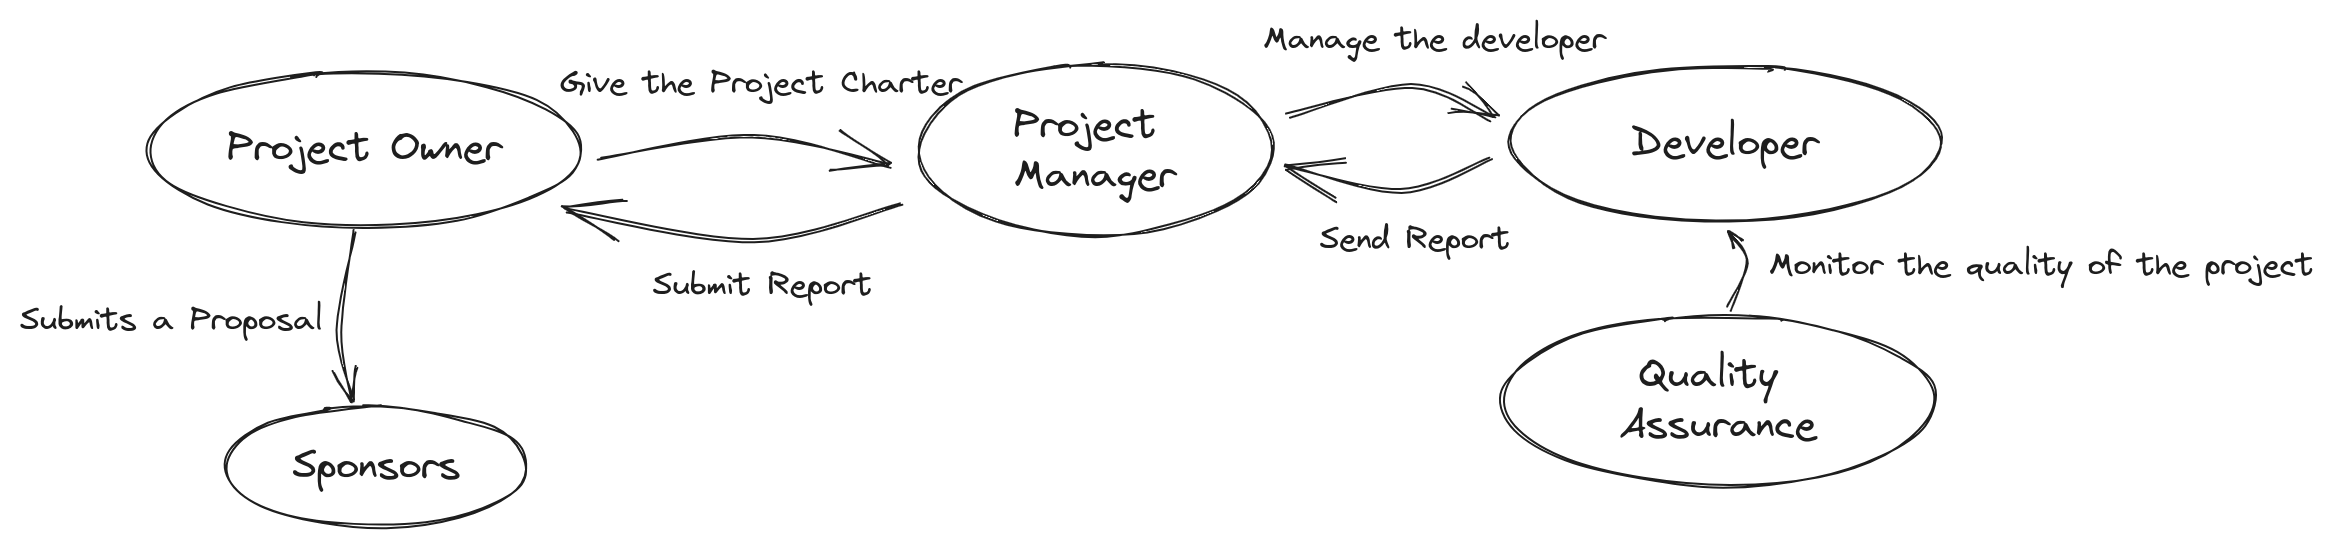
\includegraphics[height=3cm]{./images/project-flow.png}
    }
    \pagebreak
    \item {
        Jelaskan tentang proses pelaksanaan manajemen proyek.
        Jelaskan pula input dan output dari tiap proses tersebut! 
        \begin{itemize}
            \item {
                \textbf{Initialisation Phase}
                \begin{itemize}
                    \item Input: Ideas from the Project Owner
                    \item Output: Project Proposal, Project Charter
                \end{itemize}
            }
            \item {
                \textbf{Planning Phase}
                \begin{itemize}
                    \item Input: Project Charter
                    \item Output: Project Implementation Plan, Work Breakdown Structure, Gantt Chart, Project Schedule, etc
                \end{itemize}
            }
            \item {
                \textbf{Execution Phase}
                \begin{itemize}
                    \item Input: Project Implementation Plan, Work Breakdown Structure, Gantt Chart, Project Schedule, etc
                    \item Output: Project Report, The Project itself
                \end{itemize}
            }
            \item {
                \textbf{Monitoring and Controlling Phase}
                \begin{itemize}
                    \item Input: Project Report, The Project itself
                    \item Output: Quality Assurance Report
                \end{itemize}
            }
            \item {
                \textbf{Closing Phase}
                \begin{itemize}
                    \item Input: Quality Assurance Report
                    \item Output: Project Report
                \end{itemize}
            }
        \end{itemize}
    }
    \item {
        Apa kaitannya antara pelaksanaan manajemen proyek dengan 9 knowledge areas of project management?

        The correlation between the implementation of project management and the 9 knowledge areas of project management is that the implementation of project management is the process of managing the 9 knowledge areas of project management.
        The 9 knowledge areas of project management is what the project manager needs to manage in order to successfully
        complete the project.
    }
\end{enumerate}

\end{document}

